\documentclass[twocolumn,onesided,9pt]{article}

\usepackage{./Task32FlyerLatexStyle/Task32Flyer}
\usepackage{todonotes}

%% -----------------------------------
%% Document information
%% -----------------------------------
\def\pubdate{DRAFT 26 June 2020}
\title{A Review of Guidance for Using Ground-Based Vertically-Profiling Wind Lidar For Wind Resource Assessment}
\shorttitle{Vertically-Profiling Wind Lidar For Wind Resource Assessment in 2020}
%\DOI{10.5281/zenodo.3862384}
\DOI{10.5281/zenodo.xxxxxxx}
\addbibresource{bibliography.bib}

\newcommand{\conceptDOI}{http://dx.doi.org/10.5281/zenodo.3862384}

%% ===================================
%% Document - specific commands
%% ===================================
%\usepackage[export]{adjustbox}
\newcommand{\IEARP}{\emph{RP-15}}
\newcommand{\IEARPn}[1]{\IEARP\ \emph{RP #1}}
\newcommand{\IEARPnote}[1]{\IEARP\ \emph{Note #1}}
\newcommand{\IEARPndetails}[2]{\IEARP,\ \emph{RP #1:\ `#2'}}
\newcommand{\IEARPnotedetails}[2]{\IEARP,\ \emph{Note #1:\ `#2'}}

%% ===================================
%% Document starts
%% ===================================
\begin{document}
	
	%% -----------------------------------
	%% Title
	%% -----------------------------------
\maketitle
\thispagestyle{cover}
	
%% -----------------------------------
%% Introductory text
%% -----------------------------------
\noindent{\Large
What is the best practice for using wind lidar for wind resource assessments in 2020?}
\vskip 6pt
	
Wind lidar are often used to supply the wind data needed for wind resource assessments. In this review we give our perspective on best practices when deploying vertically-profiling wind lidar for wind resource assessments in 2020. This document is particularly aimed at new wind lidar users.
	
%% -----------------------------------
%% Why
%% -----------------------------------
\subsection*{Our goal}
Our goal is to document the steps required to collect high-quality, well-documented wind lidar data for use in wind resource assessments on land.
	
\subsection*{Our use case}
We focus on ground-based lidar that use a fixed scan geometry to deliver data that are to be used in the resource assessment phase of a wind farm development on land. These data typically consist of vertically-resolved profiles of wind speed and direction.

\subsection*{A short history of guidance documents}
In 2013 IEA Wind Task 32 and Task 11 published their recommended practices for ground-based remote sensing for wind resource assessment \cite{RP15_2013}, known as \IEARP. It was published to satisfy a need from the wind energy community for documented good practice in measurements with active remote sensing devices (RSDs), including lidar and sodar. \href{https://github.com/IEA-Wind-Task-32/RP15-Ground-Based-Remote-Sensing-for-Wind-Resource-Assessment/releases/tag/1.0}{It is still available online}.

\IEARP provided specific guidance as ``Recommended Practices'' (e.g., \IEARPn{1}) and informative notes (e.g. \IEARPnote{1}) about how to use remote sensing. These covered many different aspects of the remote sensing lifecycle. The document was based on experience and collected the remote sensing community's understanding in 2013. Therefore it was not a standard, but a ``recommended practices'' document.

In 2016, the Measuring Network of Wind Energy Institutes - MEASNET - published Version 2.0 of a \emph{``Procedure for the evaluation of site-specific wind conditions''} \citep{Measnet_SiteAssessment_2016}. This procedure provides generic guidance to measuring wind characteristics, and a normative annex on wind measurement using remote sensing devices. It also includes guidance on how to set up measurement campaigns depending on the data required. It is available from \href{http://www.measnet.com/wp-content/uploads/2016/05/Measnet_SiteAssessment_V2.0.pdf}{www.measnet.com}.
  % 6140-12-7

In 2017 the International Electrotechnical Committee published a new edition of the IEC 61400-12-1 `Standard for power performance testing of wind turbines' \citep[IEC 61400-12-1 (2017), ][]{IEC_61400_12_1_2017}. The IEC 61400-12-1 standard has traditionally been used as a \emph{de facto} standard for the measurements required for a wind resource assessment. It includes Annex L on the use of remote sensing for wind measurements. As a result, some groups also consider this standard to be applicable to the use case we consider here. The IEC 61400-12-1 (2017) standard can be \href{https://webstore.iec.ch/publication/66163}{purchased from the IEC}.

\section*{Motivation for this review}

So, which of these documents are still applicable? This document provides a short update of what we consider to be `best practice` in 2020. It is particularly aimed at new wind lidar users.

%% -----------------------------------
%% What to do in 2020
%% -----------------------------------
\section*{What to do in 2020}
The following sections identify the documents that are applicable at different steps in the lifecycle of a wind lidar deployment. They include:
	
\begin{itemize}
	\item \S \ref{sec:characterizing} Characterising wind lidar
	\item \S \ref{sec:installing} Installing wind lidar
	\item \S \ref{sec:operating} Operating wind lidar
	\item \S \ref{sec:analysis} Lidar data analysis
	\item \S \ref{sec:verification} Verification of wind lidar.
\end{itemize}
	
	%% -----------------------------------
	%% Characterising RSD (RP1)
	%% -----------------------------------

\section{Characterising wind lidar}
\label{sec:characterizing}
It is important that the technology used in the lidar is well characterized for future reference. This is covered in \IEARPndetails{1}{Documentation of RSD characteristics}.

%% -----------------------------------
%% Installing RSD (RP2-16)
%% -----------------------------------

\section{Installing wind lidar}
\label{sec:installing}
\subsection{Training}
Users are encouraged to take specialist training on the wind lidar before deploying the device. This is covered in \IEARPndetails{2}{Training of workers}.

\subsection{Selecting lidar deployment sites}
Careful site selection is important to get high-quality data. The user should:

\begin{itemize}
\item \textbf{Choose a representative location} that takes into account how the lidar data will be used. This should be done in collaboration with stakeholders. Possible approaches are discussed in the MEASNET document \citep{Measnet_SiteAssessment_2016}.
\item \textbf{Avoid obstructions.} Wind lidar should have a clear sky view. This is described in \IEARPn{6 d}. Some lidar devices can deliver accurate data when the beams are partially obstructed.
\item \textbf{Avoid small-scale wind disturbances} such as mast or tower wakes or other phenomena that might pass through the measurement volume, but are not related to the wind resource that a wind turbine would experience. \IEARPn{6 c} recommends avoiding such features. Some wind lidar devices include ignore data processing that can filter out the effects of such small-scale wind disturbances.
\end{itemize}
  
Because data processing tools are specific to each device, users should always follow the manufacturer's guidance on how to site their device.

\subsection{Deploying wind lidar in complex terrain}
\label{sec:complex}
Terrain influences the winds above it. This can lead to changes in flow within the lidar's measurement volume. This terrain-induced, measurement-scale flow inhomogeneity is often referred to generally as `complex flow' that occurs in `complex terrain'. It is important to note that flow conditions are also influenced by many other factors beside the terrain form. These may include land cover, measurement height, and weather \cite[amongst others; see e.g.,][]{Clifton_2015_a}

Lidars and cup anemometers use different wind measurement principles. A lidar measurement is based on information from an extended measurement volume, while a cup anemometer uses data from one point. In complex flow, wind lidar and cup anemometers will therefore give somewhat different data.

Cup anemometers are the accepted reference device for the wind energy industry. Therefore, `transfer methods' have been developed between wind lidar and cup anemometers. These use many different approaches and are often device-specific. The applicability or suitability of these methods is out of scope for this document.

Users may still wonder, ``when might the flow be complex enough to need a transfer method?''. There is no directly applicable standard because of the range of devices and transfer methods. Therefore, we suggest that it may be appropriate to work with lidar vendors and other experts to assess the need for a transfer method if conditions are complex according to IEC 61400-12-1 (2017).

The use of transfer methods should also be driven by the purpose for which the data is being used. Lidar users should always work with their stakeholders to understand their requirements. This may also have implications for verification.

An IEA Wind Task 32 working group on the use of wind lidar in complex terrain is carrying out a group study on several different transfer methods. Results are expected in 2021, and the group may publish guidelines based on their experience.

\subsection{Transport}
Suggestions for how to prepare and transport lidar are given in \IEARPndetails{4}{Reusable protective packaging for RSD transport} and \IEARPndetails{5}{Installation of shock detectors on the RSD}.
	
\subsection{Site preparation}
Recommendations for site preparation to help ensure a successful deployment are given in \IEARPn{6 a and b}.
	
\subsection{Lidar orientation}
It is important to document the lidar's compass orientation. Recommended practices are given in \IEARPndetails{7}{Device alignment}.
	
\subsection{Tilt and roll}
It is important to monitor the lidar's tilt and roll with respect to  vertical. This may be required for data analysis or to monitor the lidar's stability. Recommended practices are given in \IEARPndetails{8}{Device leveling} and \IEARPndetails{9}{Tilt sensors on the RSD}.
	
\subsection{Time synchronization}
Comparing data from multiple sources (for example, a wind lidar and a traditional tower) requires that the different data be sychronized. Appropriate recommended practices are given in \IEARPndetails{10}{Time sychronization}.
	
\subsection{Power supply}
Many wind lidar devices will be deployed `off the grid'. Recommendations on how to choose a power supply option for such situations are given in \IEARPndetails{11}{Design of remote power systems}. Remote power systems that have any kind of on-site fuel require special care and preparation. Recommended practices are given in \IEARPndetails{12}{Fuelled remote power systems}.
	
\subsection{Protection from interference}
Like any unattended equipment, care should be taken to protect a ground-based lidar from interference. This is covered in \IEARPndetails{13}{Protection from interference}.
	
\subsection{Safety signs and interlocks}
The need for safe operation and signage is covered in \IEARPndetails{14}{safety signs, interlocks and operation}.
	
\subsection{Function check}
It is important to check that the lidar is working properly before being left unattended. A checklist was suggested in \IEARPndetails{15}{Function checklist}. These checks are still useful, but now might be implemented as part of automated tests by the lidar.

\subsection{Stakeholder-driven documentation}
An installation report can add value to the final data set that is used in the wind resource assessment by reducing uncertainty.

The user should check that the information in the installation report satisfies their stakeholders and considers future needs. Many vendors and third-party engineers provide templates to help collect this data.  \IEARPndetails{16}{Installation report} also suggests a list of things to include in an installation report.


%% -----------------------------------
%% Operating wind lidar
%% -----------------------------------

\section{Operating wind lidar}
\label{sec:operating}
\subsection{Communications}
\IEARP\ gives recommendations for how to provide remote access to a wind lidar (\IEARPndetails{17}{Remote access to the RSD}).

%\subsection{Quantifying sensitivity to ambient conditions}


%If they need such information for their specific use case, lidar users can request a sensitivity analysis that documents the performance of the lidar according to IEC 61400-12-1 (2017) Annex L from the lidar vendor or through a third party. Users should then collect relevant weather data at the deployment site.

\subsection{Deployments in cold climates}
Wind lidar can be deployed in cold climates. In icing conditions they may be easier to keep in operation than wind measurement towers, or could be used together to increase data availability. Like any equipment deployed in cold climates, wind lidar need a reliable power supply, as described in  \IEARPndetails{11}{Design of remote power systems}.

There is an ongoing IEA Wind Task 32 and Task 19 joint effort to share and document experience in using wind lidar in cold climates. Results are expected in 2021 and may lead to the publication of guidelines for this use case.


\subsection{Servicing and maintenance}
Like all wind measurement devices, wind lidar may require maintenance from time to time. Recommendations for how wind lidar users and suppliers can work together to ensure reliability and repeatability are provided in \IEARPndetails{23}{Recommended service intervals}.

\subsection{Operation and maintenance log}
Users should keep a log of all use and maintenance of the wind lidar. This is described in \IEARPndetails{24}{Operation and maintenance log}.

%% -----------------------------------
%% Remote sensing data analysis (RP 25-29)
%% -----------------------------------
\section{Remote sensing data analysis}
\label{sec:analysis}

\subsection{Wind speed and vector}
It can be helpful to save data wind lidar data at different steps in the internal data processing. Recommendations for what data to store are given in \IEARPndetails{25}{Line-of-sight wind velocity}, \IEARPndetails{26}{Instantaneous wind vector}, and \IEARPndetails{27}{Time-averaged wind vector}.

\subsection{Turbulence intensity}
Sometimes, lidar users wish to collect turbulence intensity (TI) data as part of a wind resource measurement campaign. These might be used to judge the suitability of a site for a specific wind turbine, or to establish the site class according to a standard. TI data can also be obtained from cups, models, and wind speed data, amongst many other methods.

Because wind lidar measures wind in a volume, there may be differences between the turbulence intensity measured by a wind lidar and that measured by a cup anemometer \citep[see e.g.,][]{clifton_2018_a}. As with complex flows (\S \ref{sec:complex}), deriving turbulence intensity from wind lidar is therefore a device-specific challenge.

There have been efforts to create transfer functions for turbulence intensity, but their applicability and suitability is out of the scope of this document. Lidar users should therefore ask vendors or consultants for guidance.

There are ongoing industry initiatives to explore the use of turbulence data from wind lidar:
\begin{itemize}
  \item The Consortium for the Advancement for Remote Sensing (CFARS, \href{http://www.cfars.org}{www.cfars.org}) is testing several methods of processing wind lidar data to estimate the turbulence intensity that a cup anemometer would measure. Results are expected in 2020.
  \item DNV-GL initiated a joint industry project (JIP; see \href{https://www.dnvgl.com/news/dnv-gl-launches-new-joint-industry-project-to-cut-wind-energy-costs-through-lidar-measurements-154393}{www.dnvgl.com}) to support acceptance and adoption of wind lidar for wind turbulence measurements. The JIP is expected to generate results in 2020 and beyond.
\end{itemize}

\subsection{Extreme gusts}
Wind resource assessment campaigns sometimes aim to provide the data used to estimate extreme wind gusts. These data are required to assess the suitability of wind turbines for the conditions at a site. Extreme gusts can be measured directly \citep[see IEC 61400-12-1 (2017)][]{IEC_61400_12_1_2017} or derived from other data.

Wind lidar and cup anemometers use different measurement principles and so extreme gusts measured by wind lidar can differ from those measured by cup anemometers. These differences are also device-specific. Therefore, users should engage with vendors and consultants if they wish to use lidar-derived data to estimate extreme gusts.

%% -----------------------------------
%% Verification of remote sensing devices (RP 30 - 41)
%% -----------------------------------
	%
\section{Verification of remote sensing devices}
\label{sec:verification}
Verification is the act of quantifying the performance of a device against a reference. Like cup anemometers and other measurement devices used in the development of wind energy facilities, the verification of a wind lidar should be driven by the user's requirements. This was discussed in \IEARP\ \emph{Section 1.7 ``A note on `bankability'''}. Verification can therefore take many forms:

\begin{itemize}
  \item Most lidars are checked by the manufacturer before delivery to customers. This can take the form of a short measurement campaign where the lidar measures winds near a reference anemometer mounted on a tall tower. A comparison of the results shows if the device is performing as expected. This comparison could be carried out according to the IEC 61400-12-1 (2017) standard \cite{IEC_61400_12_1_2017}. Alternatively, the lidar can be placed next to another lidar that is regularly compared to a cup anemometer on a mast. These pre-delivery tests are the same concepts as those offered for cup anemometers.
  \item Users who want to explore the performance of a lidar device could use the approaches set out in \IEARPn{30 -- 40}. However, \IEARP\ is unlikely to provide the information needed for an investment decision.
  \item Users who require more detailed information about the device uncertainty -- for example as part of the financing package for a wind energy facility -- might require an uncertainty certification according to the IEC 61400-12-1 (2017) standard \cite{IEC_61400_12_1_2017}.
\end{itemize}

These methods may give slightly different uncertainty estimates and the results may be treated differently by different stakeholders. Users should therefore work closely with stakeholders to ensure that they choose a verification approach that gives them an appropriate uncertainty budget.

Verification guidelines for remote sensing devices are being reviewed by the IEC as part a new wind measurement standard (IEC 61400-50-2). This standard is expected in 2020 or 2021.

\section*{Summary}
Many groups have published guidance about the use of wind lidar for wind resource assessment.

Many of the recommendations made in the 2013 IEA Wind \IEARP\ are still applicable in 2020, particularly in relation to general good practice when deploying, operating, and maintaining wind lidar.
	
Since 2013 the wind energy community has gathered a huge amount of experience in using wind lidar data. Some of this experience has been captured in MEASNET \cite{Measnet_SiteAssessment_2016} and in the IEC 61400-12-1 Standard for power performance measurements \cite{IEC_61400_12_1_2017}.

Upcoming new IEC standards for resource assessment, instrumentation and measurements -- to be published in the 2020s -- may in turn deprecate these documents. Similarly, coordination across the wind lidar community and wind-energy industry initiatives ( Task 32, CFARS, DNV-GL, IEC, and others) may lead to convergence on methods.

%% -----------------------------------
%% Feedback
%% -----------------------------------

\section*{Your feedback and comments}
We welcome constructive feedback about this review and other IEA Wind Task 32 activities. Feedback about this review should be directed to \href{https://github.com/IEA-Wind-Task-32/RP15-status-update}{the review's GitHub repository} or to the \href{mailto:ieawind.task32@ifb.uni-stuttgart.de}{Task 32 Operating agents}.

We anticipate revising this document during the years 2021-2023 to reflect feedback and new developments. Check for revisions at \href{\conceptDOI}{\conceptDOI}.

	
    %% -----------------------------------
    %% References
    %% -----------------------------------
    %\subsection*{References}
    % bibliography
    \label{sec:References}
    \addcontentsline{toc}{section}{References}
    {\small
    \printbibliography
    }
    \vspace*{\fill}


    %% -----------------------------------
    %% Outlined block of smaller text
    %% -----------------------------------
\begin{tcolorbox}[width=1.0\columnwidth,
	boxsep=0pt,
	left=3pt,
	right=3pt,
	top=3pt,
	arc=0pt,
	boxrule=0.5pt,
	toprule=0.5pt,
	colback=white,
	coltext=TextGrey
	]
{%
%% -----------------------------------
%% IEA WIND AND TASK 32
%% -----------------------------------
\noindent%
\footnotesize%
\begin{center}%
\vspace{-2mm}
\begin{tabular}{m{0.3\columnwidth}m{0.6\columnwidth}}
\multicolumn{2}{m{\dimexpr0.9\columnwidth+2\tabcolsep\relax}}{This document was self published by IEA Wind Task 32.}\\
% IEA Wind * DO NOT EDIT THIS TEXT *

\includegraphics[height=2cm]{graphics/IEAWind_logo.jpg}
&
The International Energy Agency is an autonomous organisation which works to ensure reliable, affordable and clean energy for its 30 member countries and beyond. \href{https://community.ieawind.org}{The IEA Wind Technology Collaboration Programme} supports the work of 38 independent, international groups of experts that enable governments and industries from around the world to lead programmes and projects on a wide range of energy technologies and related issues.
\\
% Task 32 * DO NOT EDIT THIS TEXT *
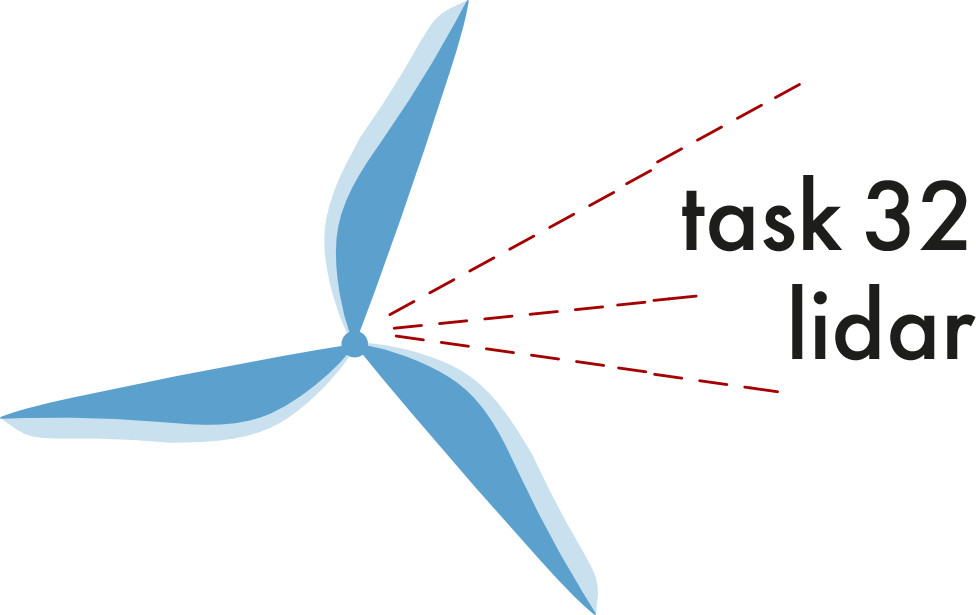
\includegraphics[height=1.5cm]{graphics/Task32_logo.jpg} &
\href{https://community.ieawind.org/task32/home}{IEA Wind Task 32} exists to identify and mitigate the barriers to the deployment of wind lidar for wind energy applications.
\\
%% -----------------------------------
%% More information
%% -----------------------------------
\multicolumn{2}{m{\dimexpr0.9\columnwidth+2\tabcolsep\relax}}{
% N.B. do not add line breaks between the next items
%% -----------------------------------
%% Authors
%% -----------------------------------
\textbf{Author team:} %
Andrew Clifton (Task 32 Operating Agent, University of Stuttgart, Germany), %
Alexander Stoekl (Energiewerkstatt), %
Nicolas Jolin (Nergica),
Paul Mazoyer (Vaisala),
Peter Clive (Black \& Veatch)
%% -----------------------------------
%% Reviewers
%% -----------------------------------
\textbf{Reviewers:} %
aaa (org x), %
bbb (org y).
%% -----------------------------------
%% Images
%% -----------------------------------
\textbf{Image credits:}
Banner, left to right: \href{https://unsplash.com/@alexkixa}{Alexandre Debiève on Unsplash}, \href{http://ifb.uni-stuttgart.de}{SWE U. Stuttgart}, \href{https://unsplash.com/@markusspiske}{Markus Spiske on Unsplash}.
} % end of more information
\end{tabular}
\end{center}
} % end of footnotesize
\end{tcolorbox} % end of tcolorbox
%% -----------------------------------
%% End of highlighted block
%% -----------------------------------
\vspace*{\fill}

\end{document}
